\section{Results and discussion}\label{results}
This section presents the results of the Austrian case study. Four different storylines are investigated, covering a wide range of possible future developments of the Austrian energy system in the context of European deep decarbonization. Section \ref{res:1} shows the heat generation mix supplying the heat demand (residential and commercial) on the country level. In Section \ref{res:2}, the obtained heat generation mix is described on finer geographical scale, sub-regional and community level. Potentials of centralized heat network are presented further in Section \ref{res:3}. Section \ref{res:4} shows the centralized heat networks on the community level. Finally, Section \ref{res:5} compares the projected centralized heat networks in 2050 with today's networks based on heat density.

\subsection{Heat supply of the Austrian residential and commercial sector in 2050: four different decarbonization scenarios obtained from the H2020 project openENTRANCE}\label{res:1}
This section presents the heat generation mix covering the Austrian residential and commercial heat demand in 2050 for four different storylines, which were (\textit{or "are currently"}) developed within the H2020 openENTRANCE project. They are named as follows: \textit{Directed Transition}, \textit{Societal Commitment}, \textit{Techno-Friendly}, and \textit{Gradual Development}. Within each of them, specific fundamental development of the energy systems is described while aiming for a sustainable transition of the provision of energy services. The first three storylines consider the achievement of the \SI{1.5}{\degreeCelsius} global warming climate target. The latter storyline (\textit{Gradual Development}) can be interpreted as a more conservative storyline aiming for the less ambitious \SI{2.0}{\degreeCelsius} climate target. Below, the storylines are briefly described before the quantitative results on the country level are presented. For a more detailed description of the storylines, it is referred to \cite{auer2020quantitative} and \cite{auer2020development}. Further informations also are available on the website of the project \footnote{\url{https://openentrance.eu/}} and GitHub\footnote{\url{https://github.com/openENTRANCE}}.\newline

The underlying concept of the four storylines is a three-dimensional space spanned by the following parameters: technology, policy, and society. Each storyline describes a specific pathway to reach a decarbonized energy system taking into account a pronounced contribution of two dimensions. Regarding the third dimension, a development is assumed that leads to no significant contribution to the decarbonization of the energy system. 

\begin{itemize}
	\item \textit{Directed Transition} looks at a sustainable provision of energy services through strong policy incentives. This bundle of actions becomes necessary because neither the markets nor society adequately pushes sustainable energy technologies.
	\item \textit{Societal Commitment} achieves deep decarbonization of the energy system by a strong societal acceptance of the sustainable energy transition. Thereby, decentralized renewable energy technologies together with policy incentives lead to a sustainable supply of energy service needs. Parallel, no fundamental breakthroughs of new clean technologies are within sight.
	\item \textit{Techno-Friendly} describes a development of the energy system where a significant market-driven breakthrough of renewable energy technologies gives rise to the decarbonization of energy service supply. Alongside, society acceptance supports the penetration of clean energy technologies and the sustainable transition.
	\item \textit{Gradual Development} differs from the other storylines as on the one hand, this storyline only aims for the less ambitious \SI{2.0}{\degreeCelsius} climate target, and on the other hand, a little of each possible sustainable development of the energy system is described here. While all three dimensions contribute to decarbonization, they do not push it sufficiently and result in a more conservative storyline than the others.
\end{itemize}

Table \ref{tab:1} shows the heat generation by technology/source in Austria 2050 for the four different storylines. These values were obtained in course of the H2020 project openENTRANCE and are the modeling results calculated using the open-source model GENeSYS-MODv2.0 \cite{burandt2018genesys}. According to the underlying assumptions in the storylines, the heat generation of the different sources/technologies vary in some cases significantly (e.g., hydrogen-based heat generation in \textit{Directed Transition} and \textit{Gradual Development} (\SI{7.62}{TWh}) or Heat pump (ground) generation in \textit{Techno-Friendly} and \textit{Societal Commitment} (\SI{14.78}{TWh})). The gray-colored column $\Sigma$ presents the sum of heat generation using centralized heat networks, which varies between \SI{19.49}{} (\textit{Techno-Friendly}) and \SI{35.23}{TWh} (\textit{Gradual Development}).

\newcolumntype{R}[2]{%
	>{\adjustbox{angle=#1,lap=\width-(#2)}\bgroup}%
	l%
	<{\egroup}%
}
\newcommand*\rot{\multicolumn{1}{R{45}{1em}}}
\newcommand*\rots{\multicolumn{1}{R{90}{1em}}}
\definecolor{Gray}{gray}{0.85}

\begin{table}[h] \centering
	\scalebox{0.9}{
	\renewcommand{\arraystretch}{1.35}
	\begin{tabular}{clcccccccc}
		\multicolumn{2}{c}{\thead{Heat generation\\by source in \SI{}{TWh}}} & \rot{Biomass} & \rot{Direct Electric} & \rot{Synthetic gas} & \rot{Heat pump (air)} 
		& \rot{Heat pump (ground)} & \rot{Heat storage} & \rot{Hydrogen} & $\Sigma$\\
		\midrule
		\parbox[t]{2mm}{\multirow{4}{*}{\rotatebox[origin=c]{90}{\small Storyline}}}
		& Directed Transition             & 5.37 & 2.13  & 0.36  & 22.73  & 19.50  & 14.84  & 1.03  & \cellcolor{Gray}25.90\\
		& Societal Commitment               & 5.37 & 1.98 & 1.35 & 15.71 & 21.47 & 10.58 & 2.18 & \cellcolor{Gray}29.02\\
		& Techno-Friendly              & 5.37 & 1.53  & 2.79  & 25.95  & 6.69 & 16.36 & 7.43  & \cellcolor{Gray}19.49\\
		& Gradual Development & 5.37 & 1.81 & 5.35 & 9.68 & 21.21 & 15.57  & 8.65 & \cellcolor{Gray}35.23\\
		\bottomrule
	\end{tabular}}
	\caption{Heat generation by source in TWh supplying the residential and commercial heat demand in Austria 2050 for the different scenarios. Values obtained from the H2020 project openENTRANCE and GENeSYS-MOD.}
	\label{tab:1}
\end{table}

\subsection{Heat technology generation in 2050 on different spatial granularities}\label{res:2}
Figure \ref{fig:res1} shows the heat generation per technology/source on different spatial granularities: the country (NUTS0), sub-region (NUTS3) and community (LAU) level (from left to right). The level of spatial details increases from the left to the right. In the middle, the residential and commercial heat supply in a representative rural and urban sub-region, respectively, is presented. The rural sub-region \textit{Mostviertel-Eisenwurzen} (NUTS3 code AT121) shows high shares of heat pumps (air sourced) and small-scale heat storage systems. In addition, synthetic gas and direct electric heating systems supply the heat demand. The urban sub-region \textit{South Viennese environs} (AT127) is mainly supplied by ground-sourced heat pumps, biomass, and hydrogen. Air-sourced heat pumps and again heat storage cover the remaining demand. Throughout the pie charts within the figure, shares of heat generation using centralized heat networks are indicated using blue-colored edges. On the very right, an example of the resulting centralized heat network on the community level for the four different scenarios is presented. Within the four subfigures presenting centralized heat networks (each for one storyline), the size of the points represents the amount of heat demand using centralized supply in a community. The comparably high heat demand in the \textit{Gradual Development} scenario results in an extensive centralized heat network infrastructure (see lower right subfigure in Figure \ref{fig:res1}). The other three centralized heat networks are characterized by fewer (less supplied small sub-regions) and smaller points (less supplied heat demand by the centralized heat network). Figure \ref{fig:res-comp} compares the heat generation by source between $2020$ (today) and $2050$ for the four different scenarios. The height of the bars shows the absolute differences by source between both years, whereby a negative difference indicates less heat generation by this source in 2050. The height of the bars indicates the values of the \textit{Societal Commitment} scenario since this is the scenario with the lowest total heat demand (\SI{-18.15}{TWh}). In addition, the scenario with the lowest and highest difference respectively is marked for each heat source and the total demand. For instance, the highest decrease is seen in natural gas in the \textit{Directed Transition} scenario (\SI{-53.76}{TWh}).

\begin{sidewaysfigure}
	\centering
	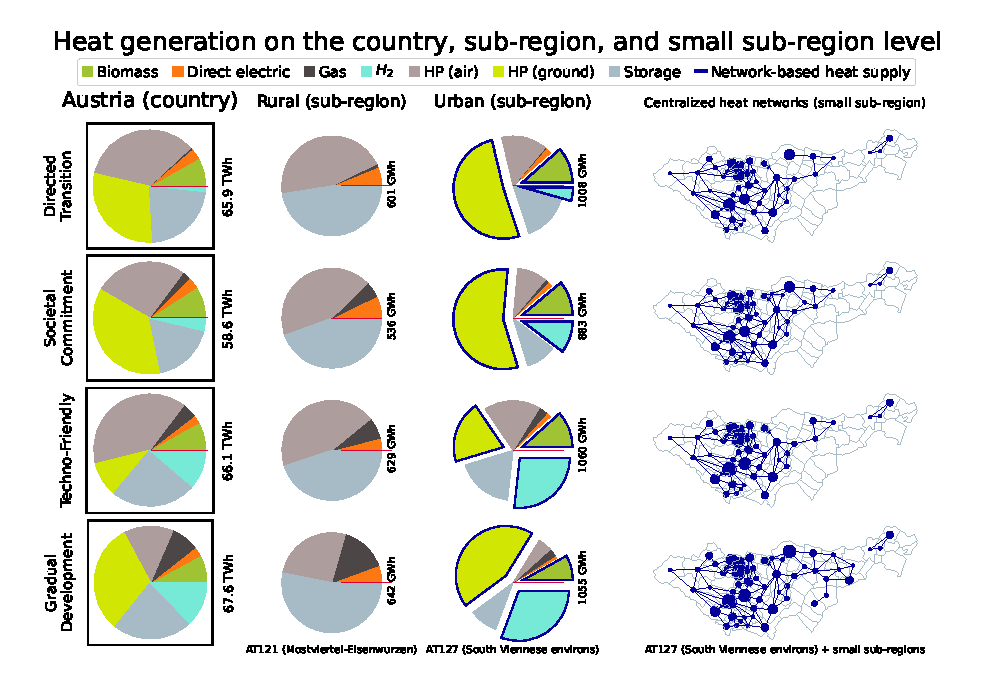
\includegraphics[width=1\linewidth]{figures/4_Results/Fig_Matrix-plot/Spatial_results.eps}
	\caption{Heat technology generation on different spatial granularity levels in the different scenarios supplying the residential and commercial heat demand. left: on the country level. middle: comparison of a rural and urban sub-region. right: centralized heat network topology (size of the points represent the amount of heat demand supplied by the network)}
	\label{fig:res1}
\end{sidewaysfigure}

\begin{figure}
	\centering
	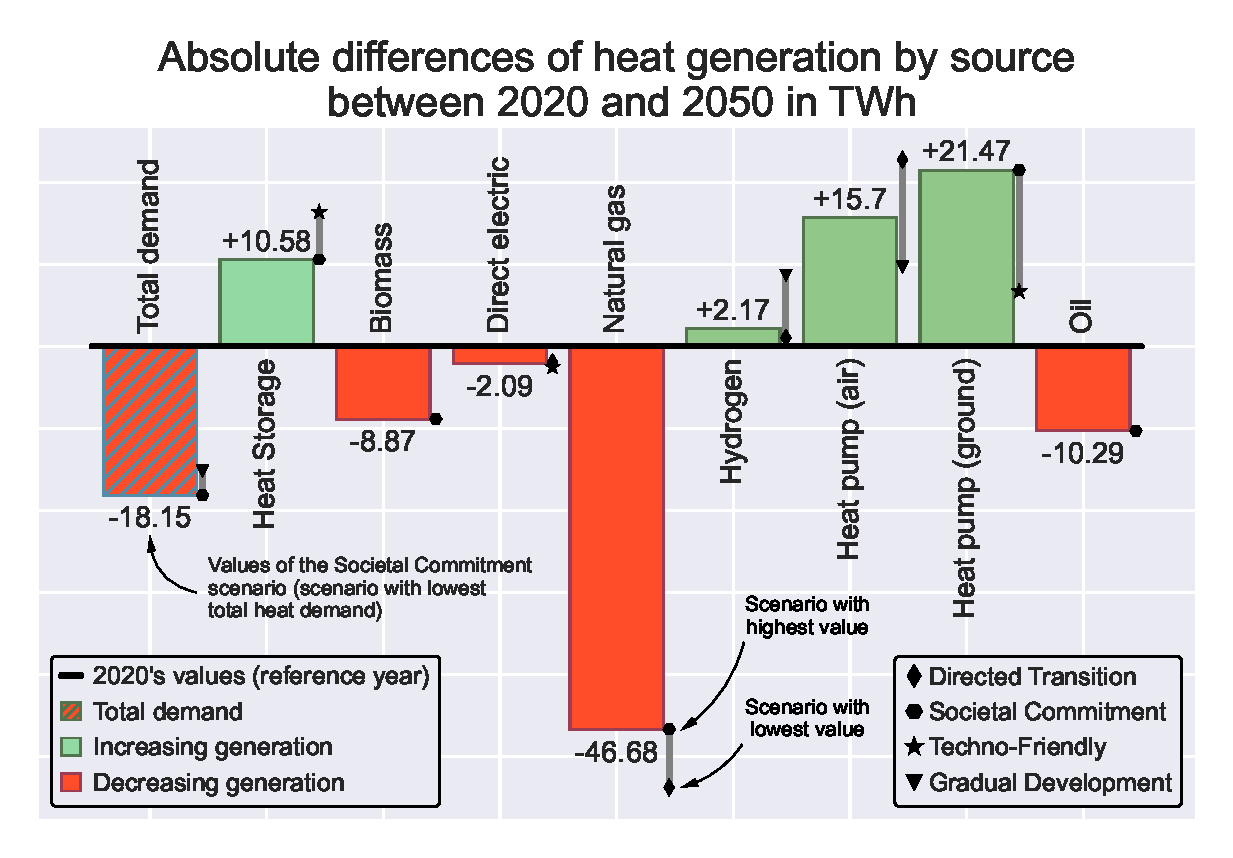
\includegraphics[width=1\linewidth]{figures/4_Results/Fig-Comp/Ref-2050.eps}
	\caption{Comparison of heat generation by source between the reference year $2020$ (black line) and 2050 in Austria. The height of the bars shows the absolute increase/decrease $2050$ in the \textit{Societal Commitment} scenario. The scenario with the lowest and highest difference, respectively, is indicated by the markers.}
	\label{fig:res-comp}
\end{figure}

\subsection{Sub-regions in Austria 2050 with high potentials for centralized heat supply}\label{res:3}
The potentials of centralized heat supply in Austria 2050 are limited to densely populated areas (urban areas). In particular, the results indicate only six different sub-regions (NUTS3 regions) that are supplied by centralized heat networks (see Figure \ref{fig:res2}). Although the exact numerical numbers differ, the six sub-regions in each scenario are (partially) supplied by centralized heat networks. Table \ref{tab:3} shows the centralized and on-site heat supply in the six sub-regions. Thereby, the connection rate is assessed by the share of centralized heat supply in the total heat demand. The population density varies in the six sub-regions between \SI{229}{persons \per \kilo\metre^2} (AT323 - Salzburg and sourroundings) and \SI{5124}{persons \per \kilo\metre^2} (AT130 - Vienna).

\begin{table} \centering
	\scalebox{1}{
		\renewcommand{\arraystretch}{1.35}
		\begin{tabular}{cccccc}
			\toprule 
			&& \multicolumn{2}{c}{in TWh} & in \%\\\cmidrule(lr){3-5}
			Sub-region & Storyline&Centralized & On-site & Connection rate\\\hline
			\parbox[t]{15mm}{\multirow{4}{*}{\rotatebox[origin=c]{90}{\parbox{2cm}{\centering South Viennesse\\environs (AT127)}}}} & Directed Transition & 0.72 & 0.17 & 81\\
			 & Societal Commitment & 0.78 & 0.11 & 88\\
			 & Techno-Friendly & 0.90 & 0.24 & 79\\
			 & Gradual Development & 1.20 & 0.09 & 93\\\hline
			 \parbox[t]{15mm}{\multirow{4}{*}{\rotatebox[origin=c]{90}{\parbox{2cm}{\centering Vienna\\(AT130)}}}} & Directed Transition & 3.98 & 0.95 & 81\\
			 & Societal Commitment & 4.28 & 0.61 & 88\\
			 & Techno-Friendly & 4.98 & 1.33 & 79\\
			 & Gradual Development & 6.59 & 0.47 & 93\\\hline
			  \parbox[t]{15mm}{\multirow{4}{*}{\rotatebox[origin=c]{90}{\parbox{2cm}{\centering Graz\\(AT221)}}}} & Directed Transition & 0.92 & 0.22 & 81\\
			 & Societal Commitment & 1.53 & 0.14 & 92\\
			 & Techno-Friendly & 1.16 & 0.31 & 79\\
			 & Gradual Development & 1.53 & 0.11 & 93\\\hline
			 \parbox[t]{15mm}{\multirow{4}{*}{\rotatebox[origin=c]{90}{\parbox{2cm}{\centering Linz-Wels\\(AT312)}}}} & Directed Transition & 1.24 & 0.30 & 81\\
			 & Societal Commitment & 1.34 & 0.19 & 88\\
			 & Techno-Friendly & 1.56 & 0.42 & 79\\
			 & Gradual Development & 2.06 & 0.15 & 93\\\hline
			  			\parbox[t]{15mm}{\multirow{4}{*}{\rotatebox[origin=c]{90}{\parbox{2cm}{\centering Salzburg and surroundings\\(AT323)}}}} & Directed Transition & 0.75 & 0.18 & 81\\
			 & Societal Commitment & 1.24 & 0.11 & 92\\
			 & Techno-Friendly & 0.93 & 0.25 & 79\\
			 & Gradual Development & 1.24 & 0.09 & 93\\\hline
			 \parbox[t]{15mm}{\multirow{4}{*}{\rotatebox[origin=c]{90}{\parbox{2cm}{\centering Rheintal-Bodensee\\(AT342)}}}} & Directed Transition & 0.66 & 0.16 & 81\\
			 & Societal Commitment & 0.71 & 0.10 & 88\\
			 & Techno-Friendly & 0.82 & 0.22 & 79\\
			 & Gradual Development & 1.09 & 0.08 & 93\\\hline
			 & & \multicolumn{2}{c}{Average connection rate}& \SI{85.25}{\%}\\
			\bottomrule
	\end{tabular}}
	\caption{Centralized heat supply and on-site heat generation in the six Austrian sub-regions, with potentials of centralized heat networks in 2050}
	\label{tab:3}
\end{table}

\begin{sidewaysfigure}
	\centering
	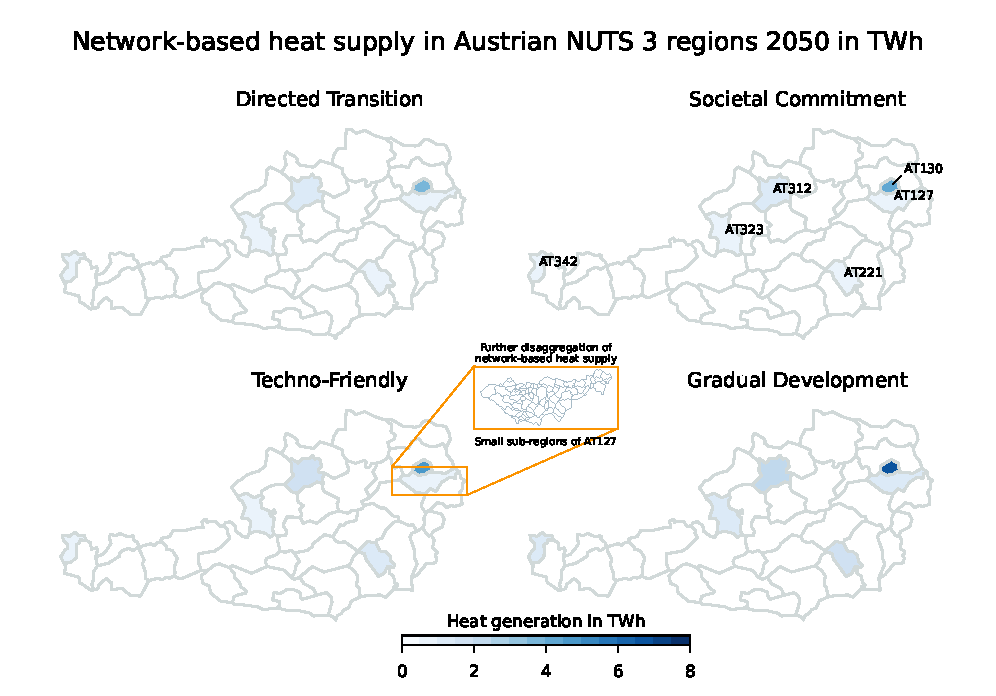
\includegraphics[width=1\linewidth]{figures/4_Results/Heatmap.eps}
	\caption{Centralized heat supply in Austria 2050}
	\label{fig:res2}
\end{sidewaysfigure}

\subsection{Centralized heat network topology on the community level}\label{res:4}
This section presents the centralized heat network topology of the sub-region \textit{South Viennese environs} (AT127) and all included communities. In Figure \ref{fig:res2}, this particular sub-region is marked by the orange box and figure \ref{fig:res3} shows the projected centralized heat network topology. In particular, the network topology is presented for the initial condition (as result of the sequential downscaling, $i=1$) and in the final condition ($i=29$) of the network. The distribution of the benchmark indicator values of the centralized heat network depending on the number of iterations is presented in the middle. Thereby, the mean value is marked in orange and increases with the number of iterations (increase from one third to almost two). Within the algorithm, this is achieved by reducing the supply area (decline in connected communities from 75 to 47). At the same time, the number of connected population decreases by \SI{13.3}{\%}, starting from a population of \SI{386}{k} being connected to centralized heating network in the before the first iteration. After the final iteration ($i=29$), the termination criterion is reached. A possible following step of iteration could not increase the benchmark indicator mean value any further. The iterative reduction of supplied small sub-regions does not necessarily result one contiguous graph. For example, three communities form a subgraph that is separate from the other network (see upper right in the final condition network graph). The results discussed above suggest that reducing the number of small sub-regions supplied by the centralized heat network increases the indicator value and thus the efficiency of the heat network topology. Simultaneously, this also increases the heat density of the supply area. In the following subsection, the obtained heat density values of the heat networks are compared with existing values and today's minimum required values for centralized heat networks.

\begin{sidewaysfigure}
	\centering
	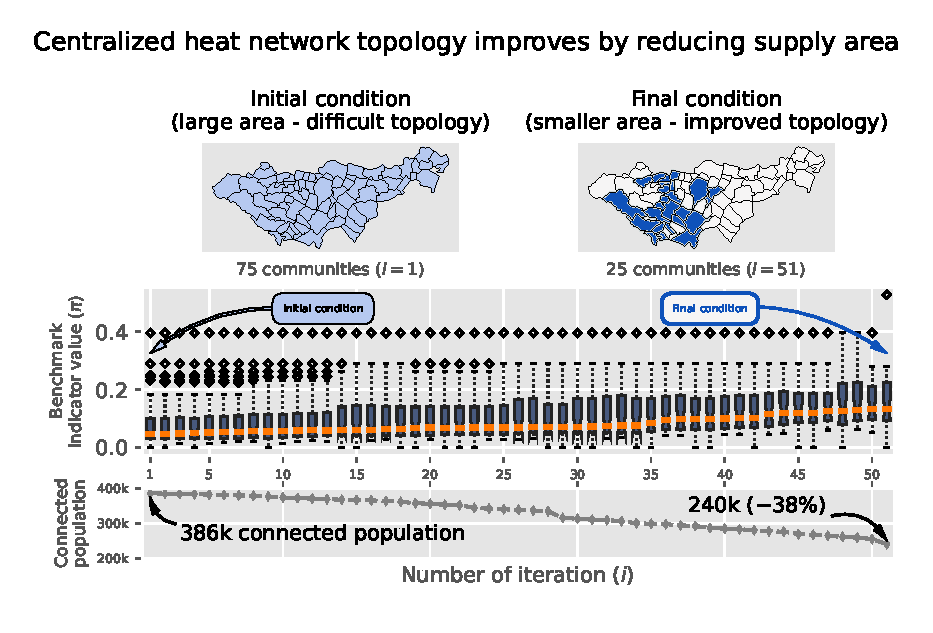
\includegraphics[width=1\linewidth]{figures/4_Results/Fig_Boxplot/ext_boxplot.eps}
	\caption{Centralized heat network topology in the initial and final condition. The boxplot (middle) indicates the improved network topology by an increasing benchmark indicator mean value (orange line). In the final condition, the connected population declines by \SI{-13.3}{\%} compared to the initial condition.}
	\label{fig:res3}
\end{sidewaysfigure}

\subsection{Comparison of 2050's and today's centralized heat networks using heat density as criterion}\label{res:5}
In the following, the centralized heat network in \textit{Graz} (AT221) is investigated in detail. Figure \ref{fig:res5} shows the heat density of the centralized heat network in the \textit{Techno-Friendly} scenario. The x-axis shows the three different downscaling techniques. The numerical numbers indicate an significant increase of the heat density resulting by the prioritized preference of heat sources (+\SI{1.07}{GWh \per km^2}) and the network topology benchmarking (+\SI{1.08}{GWh \per km^2}). However, comparing the obtained heat density value with heat density values of today's centralized heat networks reveals a signifcant gap (see the pink bar). According to references from the practice (see, e.g., in \url{http://www.austrian-heatmap.gv.at/ergebnisse/}), the heat density of today's networks is assumed to be \SI{10}{\frac{GWh}{km^2}} with a connection rate of \SI{90}{\%}. In general, the gap of heat density varies between the different scenarios. The smallest is achieved in the \textit{Techno-Friendly} scenario and amounts to \SI{7.42}{\frac{GWh}{km^2}} as presented in Figure \ref{fig:res5} by the pink bar. The largest gap is seen in the \textit{Societal Commitment} scenario and is \SI{8.41}{\frac{GWh}{km^2}}. The presented results of the sub-region are representative for the other sub-regions with potentials of centralized heat networks (excluding \textit{Vienna} (AT130)). Figure \ref{fig:res4} presents for the six different sub-regions the heat density values 2050 and the correspondig heat density gap. The heat density gap of \textit{Graz} in the \textit{Directed Transition} scenario is highlighted similar to the presentation in Figure \ref{fig:res5}. In particular, the results indicate no heat density gap for \textit{Vienna} (AT130) in all the scenarios, except a minor one in the results obtained using \textit{Directed Transition} scenario.  

\begin{figure}[h]
	\centering
	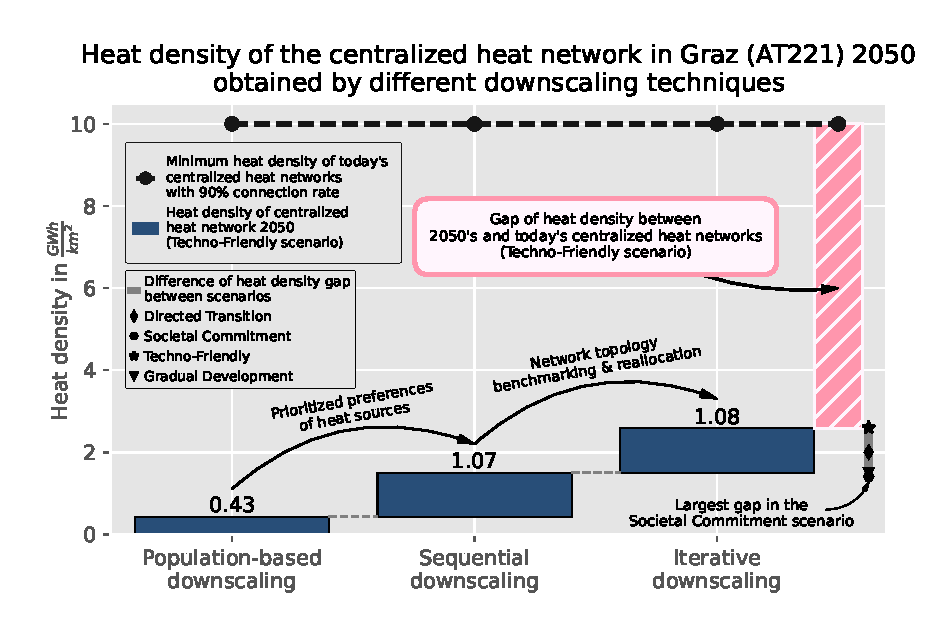
\includegraphics[width=1\linewidth]{figures/4_Results/Fig_Heat-density/HD_cleaned1.eps}
	\caption{Heat density of the centralized heat network in \textit{Graz} (AT221) 2050 in the \textit{Techno-Friendly} scenario. The gap of heat density between 2050's and today's heat density (black dashed line) is marked by the pink bar.}
	\label{fig:res5}
\end{figure}

\begin{figure}[h]
	\centering
	\includegraphics[width=1\linewidth]{figures/4_Results/Fig_Gap/HD1.eps}
	\caption{Heat densities (blue bars) of centralized heat networks in the six Austrian sub-regions and in the four different decarbonization scenarios. The heat density gap to today's centralized heat networks is indicated in pink. The smallest heat density gap (excluding \textit{Vienna} (AT130) is marked by the white hatch.)}
	\label{fig:res4}
\end{figure}